\chapter{HTTP Server}

A commonly seen Linux application is to host a web service. "LAMP", an acronym that stands for Linux, Apache, MySQL, and PHP/Perl/Python, is a classic architecture for that application. In this structure, Linux serves as the host OS for the server, Apache as the web service provider, MySQL as the backend database, and finally PHP/Perl/Python as the programming languages for web development.

Database services, both RDB such as MySQL, MariaDB, PostgreSQL and NoSQL such as MongoDB, Redis have introduced in earlier chapters. Apache HTTP server is introduced in this chapter. Programming languages such as PHP and Python are not covered in this notebook.

Notice that Apache is not the only web service provider in the market. Alternative choices include Nginx, Node.js and many other options.

\section{Brief Introduction to Apache HTTP Server}

Web server is a network services that serves content to a client over the internet. The client can be a web browser or any other software that supports the pre-agreed communication protocol, one of the most widely used ones of which is the hypertext transport protocol (HTTP). Details about HTTP protocol is not introduced in this notebook.

\textit{Apache HTTP server}, also known as \textit{httpd} in RHEL, is one of the web service providers in the market. It is an open-source web server project developed by the Apache Software Foundation. A full list of projects managed by the Apache Software Foundation can be found at \cite{apache2024projects}. Famous apache projects include Apache Spark, and many more.

This chapter introduces the basic configuration and usage of Apache HTTP server. For more details, visit the Apache HTTP Server website at \textit{https://httpd.apache.org/}. 

\section{Installation of Apache HTTP Server}

Apache HTTP server can be installed and executed on the host machine or deployed in a container.

\subsection{Apache HTTP Server Installation on Host Machine}

The package for Apache HTTP server on RHEL repositories is \verb|httpd|. To install Apache HTTP server on RHEL, use
\begin{lstlisting}
$ sudo dnf install httpd
\end{lstlisting}

To start and enable \verb|httpd|, use
\begin{lstlisting}
$ sudo systemctl start httpd
$ sudo systemctl enable httpd
\end{lstlisting}

A testing page is provided. Upon installation, retrieve the testing page by
\begin{lstlisting}
$ curl localhost
\end{lstlisting}
and the test page HTML will show up in the console. Alternatively, use a web browser to visit the host server at port $80$ to see the web page visually that looks like Fig. \ref{ch:vac:fig:httpdtestpage}. Notice that firewall may need to be configured to allow HTTP TCP access on port $80$, which can be done by
\begin{lstlisting}
$ sudo firewall-cmd --permanent --add-port=80/tcp
$ sudo firewall-cmd --reload
\end{lstlisting}
Firewall configurations will be introduced in more details in later part of the notebook under Linux security.

\begin{figure}[htbp]
	\centering
	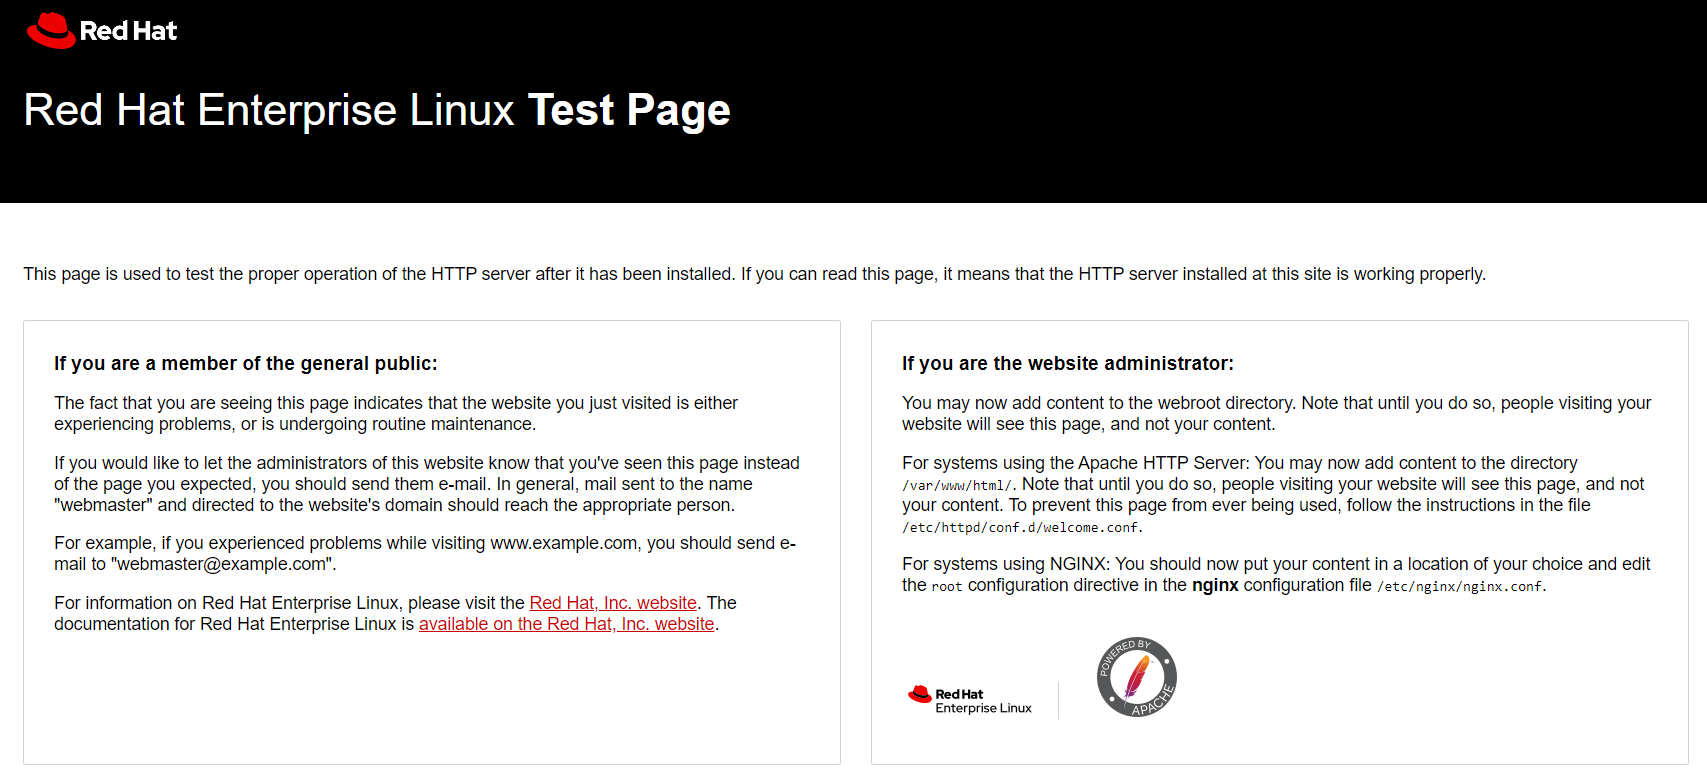
\includegraphics[width=350pt]{chapters/part-3/figures/httpdtestpage.png}
	\caption{Apache HTTP server test page on RHEL.} \label{ch:vac:fig:httpdtestpage}
\end{figure}

\subsection{Apache HTTP Server in Container}

Apache HTTP server also has a Docker image, and it can run in a container. More information can be found at \cite{docker2024httpd}. In short, one can build the image using the following Dockerfile 
\begin{lstlisting}
FROM httpd:latest
COPY ./public-html/ /usr/local/apache2/htdocs/
\end{lstlisting}
followed by
\begin{lstlisting}
$ docker build -t <image name> .
$ docker run -dit --name <container name> -p 8080:80 <image name>
\end{lstlisting}
where \verb|./public-html/| is a directory on the host machine that contains all the HTML files. Alternatively, download and run the image from Docker Hub by
\begin{lstlisting}
$ docker run -dit --name <container name> -p 8080:80 -v "$PWD":/usr/local/apache2/htdocs/ httpd:latest
\end{lstlisting}

In the remaining of this chapter, we assume that Apache HTTP server is installed on the host machine. With that being said, all the configurations and functions should work similarly if it were run in a container.

\section{Apache HTTP Server Configuration and Deployment}

Configuration files setup the environmental variables (such as the location of the web pages, the port number, etc.) and control the behavior of the web server. Apache HTTP server configuration files include
\begin{itemize}
	\item \verb|/etc/httpd/conf/httpd.conf|: the main configuration file
	\item \verb|/etc/httpd/conf.d/|: an auxiliary directory of configurations files included in the main configuration file
	\item \verb|/etc/httpd/conf.modules.d/|: an auxiliary directory that contains configuration files for modules
\end{itemize}

Commonly used configurations are introduced in this section.

\subsection{Virtual Host Configuration}

\begin{shortbox}
	\Boxhead{Default Host VS Virtual Host}
	
	By default, an HTTP server deploys one website and all the website contents such as HTML files, JavaScript files and CSS files shall be stored in \verb|/var/www/html/|. The idea of virtual host is to enable one HTTP server to deploying multiple websites, each stored in their associated subdirectory \verb|/var/www/html/<virtual host name>/|. The virtual host information such as the port number, document root, etc., needs to be configured in \verb|httpd.conf| the main configuration file.
	
	Even if deploying only one website, it is still rather a good practice to use a virtual host than to use the default host for consistency and ease of management.
\end{shortbox}

To deploy a virtual host, the main configuration file \verb|httpd.conf| shall be appended with the following content.
\begin{lstlisting}
<VirtualHost *:80>
	ServerAdmin <username>@example.com
	ServerName example.com
	DocumentRoot /var/www/html/example
	ErrorLog /var/log/httpd/example_error.log
	CustomLog /var/log/httpd/example_access.log combined
</VirtualHost>
\end{lstlisting}
where \verb|example| and \verb|example.com| can be replaced with the website name. Note that this is only a simple configuration with only the document root location, server name, and log locations. A practical virtual host configuration is usually more complex and filled with more details such as security policies, etc.

It is possible to add a configuration file for the particular virtual host at \verb|/etc/httpd/conf.d/|. In this example
\begin{lstlisting}
/etc/httpd/conf.d/example.conf
\end{lstlisting}
can be created and included as part of the main configuration file. This is optional and can become useful when the configuration is complicated.

With above setup, use
\begin{lstlisting}
http://<server name>
\end{lstlisting}
to browse the virtual host, where
\begin{itemize}
	\item The \verb|<server name>| matches the \verb|ServerName| or \verb|ServerAlias| in the configuration file
	\item A DNS needs to be setup as a prerequisite, otherwise \verb|<server name>| cannot be resolved.
\end{itemize}

\subsection{Kerberos Authentication Configuration}

Kerberos is a network authentication protocol. User registration and authentication have become a widely adopted feature in modern websites so that they can distinguish and provide different contents for different users. Kerberos can be used to back up this feature. Details of Kerberos is not given in this notebook. 

RHEL uses GSS-Proxy module to provide support for Apache HTTP server running on it to perform Kerberos authentication. For that, make sure that \verb|gssproxy| package is installed. 




\section{A Brief Introduction to Website Development}










\section{Other Web Servers}